% Options for packages loaded elsewhere
\PassOptionsToPackage{unicode}{hyperref}
\PassOptionsToPackage{hyphens}{url}
%
\documentclass[
  landscape]{article}
\usepackage{lmodern}
\usepackage{amssymb,amsmath}
\usepackage{ifxetex,ifluatex}
\ifnum 0\ifxetex 1\fi\ifluatex 1\fi=0 % if pdftex
  \usepackage[T1]{fontenc}
  \usepackage[utf8]{inputenc}
  \usepackage{textcomp} % provide euro and other symbols
\else % if luatex or xetex
  \usepackage{unicode-math}
  \defaultfontfeatures{Scale=MatchLowercase}
  \defaultfontfeatures[\rmfamily]{Ligatures=TeX,Scale=1}
\fi
% Use upquote if available, for straight quotes in verbatim environments
\IfFileExists{upquote.sty}{\usepackage{upquote}}{}
\IfFileExists{microtype.sty}{% use microtype if available
  \usepackage[]{microtype}
  \UseMicrotypeSet[protrusion]{basicmath} % disable protrusion for tt fonts
}{}
\makeatletter
\@ifundefined{KOMAClassName}{% if non-KOMA class
  \IfFileExists{parskip.sty}{%
    \usepackage{parskip}
  }{% else
    \setlength{\parindent}{0pt}
    \setlength{\parskip}{6pt plus 2pt minus 1pt}}
}{% if KOMA class
  \KOMAoptions{parskip=half}}
\makeatother
\usepackage{xcolor}
\IfFileExists{xurl.sty}{\usepackage{xurl}}{} % add URL line breaks if available
\IfFileExists{bookmark.sty}{\usepackage{bookmark}}{\usepackage{hyperref}}
\hypersetup{
  pdftitle={Lets Roomie BI Dashboard},
  pdfauthor={Castor Dams},
  hidelinks,
  pdfcreator={LaTeX via pandoc}}
\urlstyle{same} % disable monospaced font for URLs
\usepackage[margin = 1.1cm]{geometry}
\usepackage{graphicx,grffile}
\makeatletter
\def\maxwidth{\ifdim\Gin@nat@width>\linewidth\linewidth\else\Gin@nat@width\fi}
\def\maxheight{\ifdim\Gin@nat@height>\textheight\textheight\else\Gin@nat@height\fi}
\makeatother
% Scale images if necessary, so that they will not overflow the page
% margins by default, and it is still possible to overwrite the defaults
% using explicit options in \includegraphics[width, height, ...]{}
\setkeys{Gin}{width=\maxwidth,height=\maxheight,keepaspectratio}
% Set default figure placement to htbp
\makeatletter
\def\fps@figure{htbp}
\makeatother
\setlength{\emergencystretch}{3em} % prevent overfull lines
\providecommand{\tightlist}{%
  \setlength{\itemsep}{0pt}\setlength{\parskip}{0pt}}
\setcounter{secnumdepth}{-\maxdimen} % remove section numbering

\title{Lets Roomie BI Dashboard}
\author{Castor Dams}
\date{28/09/2020}

\begin{document}
\maketitle

\renewcommand{\contentsname}{Indice de Indicadores}

\tableofcontents

\newpage

\hypertarget{resumen}{%
\section{Resumen}\label{resumen}}

En el presente dashboard se muestran los principales indicadores de la
plataforma de Let's Roomie.

Los datos mostrados son provenientes de la base de datos en MongoDB del
proyecto. Dichos datos fueron scrapeados de la página de renta de
apartamentos \textbf{www.fincaraiz.com.co} usando Xpath con Python.

\hypertarget{lugares-publicados}{%
\section{Lugares Publicados}\label{lugares-publicados}}

\hypertarget{distribuciuxf3n-de-precios-ofrecidos}{%
\subsection{Distribución de Precios
Ofrecidos}\label{distribuciuxf3n-de-precios-ofrecidos}}

En el siguiente histograma se muestra la distribución de precios de los
diferentes lugares ofertados en la plataforma.

\begin{center}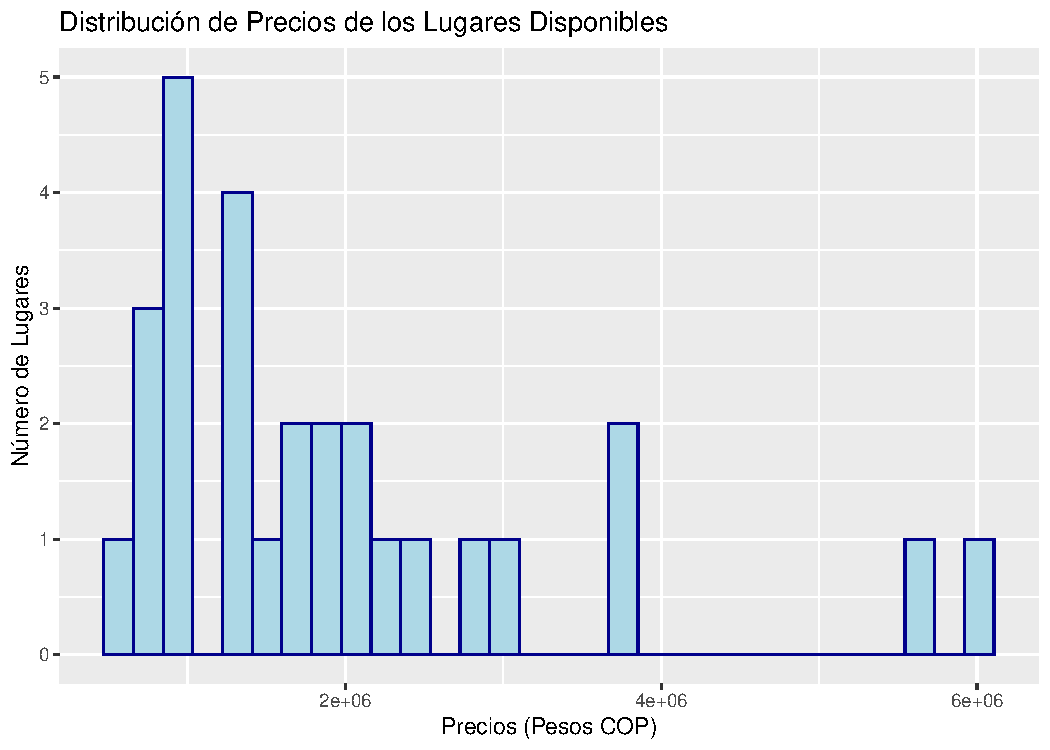
\includegraphics{BI_reporting_files/figure-latex/WebScraper_Constants-1} \end{center}

En el eje Y se muestra el numero de lugares que ofrecen ese precio y en
el eje X el Rango de los precios en Pesos Colombianos.

\hypertarget{uxe1rea-de-viviendas}{%
\subsection{Área de Viviendas}\label{uxe1rea-de-viviendas}}

\begin{center}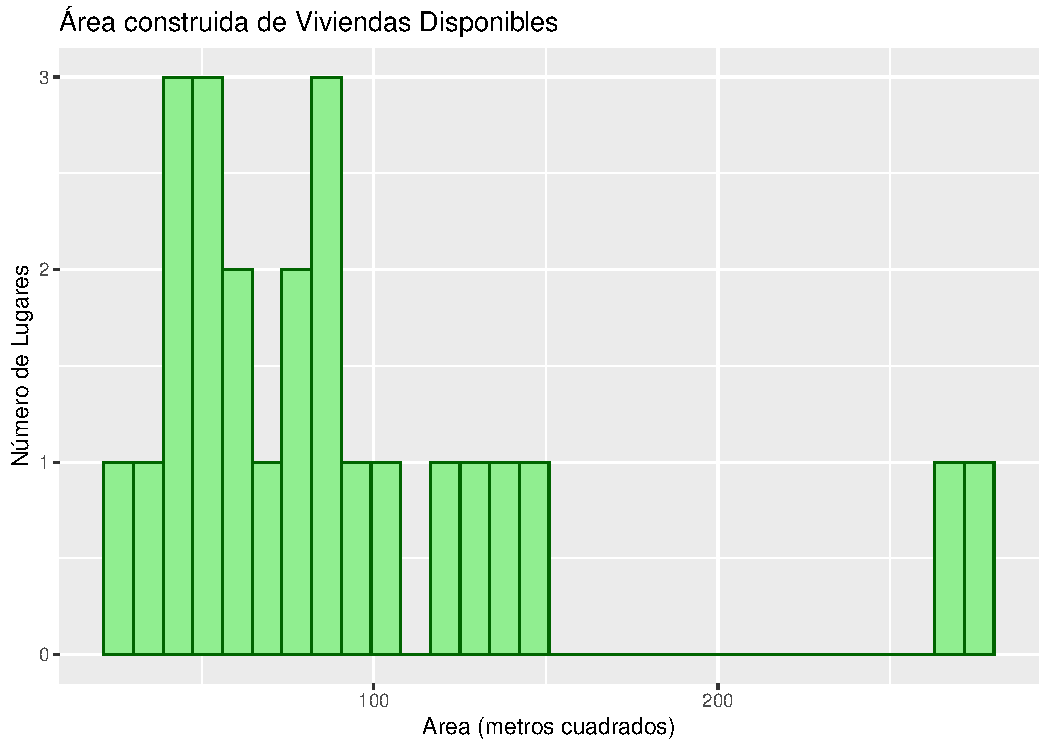
\includegraphics{BI_reporting_files/figure-latex/Grafica_superficie -1} \end{center}

El Área se refiere a la cantidad de metros cuadrados de construcción que
tiene el departamento o la casa que ofrecen los usuarios en la
plataforma.

NOTA: El área no va relacionada con el precio ofrecido en la plataforma
ya que no se toman en cuenta datos como la ubicación, los detalles de
construcción ni los servicios externos a la vivienda.

\end{document}
